\section{\xxx Overview} \label{sec:overview}

\subsection{Architecture} \label{sec:arch}

Figure 2 shows \xxx's architecture. It contains three main components.

% On receiving a packet, QEMU calls tap_send()
% On sending a packet, QEMU calls tap_receive()

The replication logic is entirely implemented in qemu-kvm, a KVM tailored version of QEMU.
We maintain a packet queue to capture outgoing packets.

\begin{figure}[t]
% \vspace{.20in}
\centering
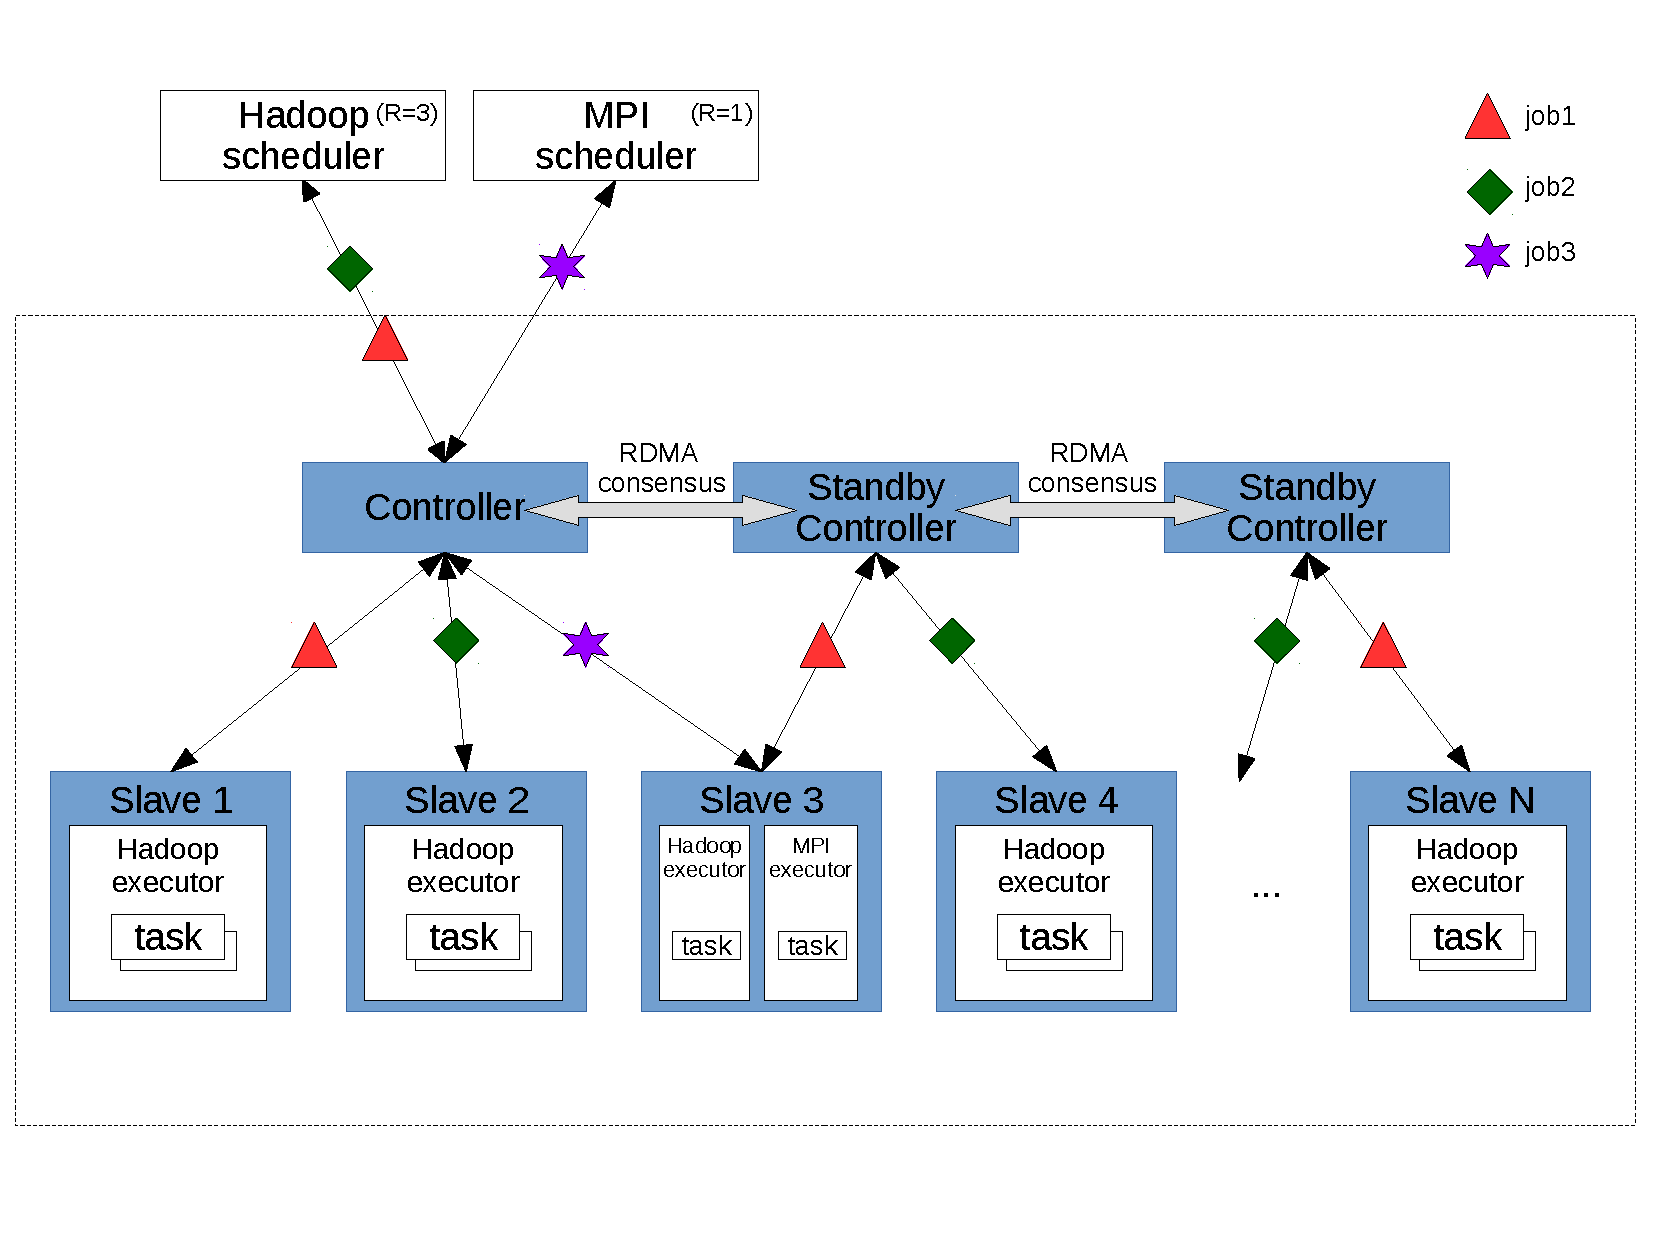
\includegraphics[width=.47\textwidth]{figures/arch}
\vspace{-.2in}
\caption{{\em The \xxx Architecture.}} \label{fig:arc}
\vspace{.05in}
\end{figure}
